% !TeX root = Stageportfolio.tex

\begin{landscape}
	
%	\begin{tabularx}{1.56\textwidth}{|X|}
%		\hline
%		Naam stagair:  Kevin Truyaert  \\
%		Tel.: 0495/928460 \hspace{3cm} e-mail: kevin.truyaert@student.kuleuven.be  \\
%		Naam en adres opleidingsinstituut:  KU Leuven Campus Kulak Kortrijk, Etienne-Sabbelaan 53, 8800 Kortrijk  \\
%		Naam directie: \\
%		Naam stagecoördinator:  David Dudal \\
%		\hline
%	\end{tabularx}
	\vspace*{-0.4cm}
\section{Observatie- en stageplanning}
\vspace*{-0.3cm}\subsection{Observatieplanning}
\subsubsection{Kulak (LIO)}%
\vspace*{-0.5cm}
%\parskip 
%\vspace{\parskip}
%\begin{minipage}[b]{\textwidth}
\begin{center}
		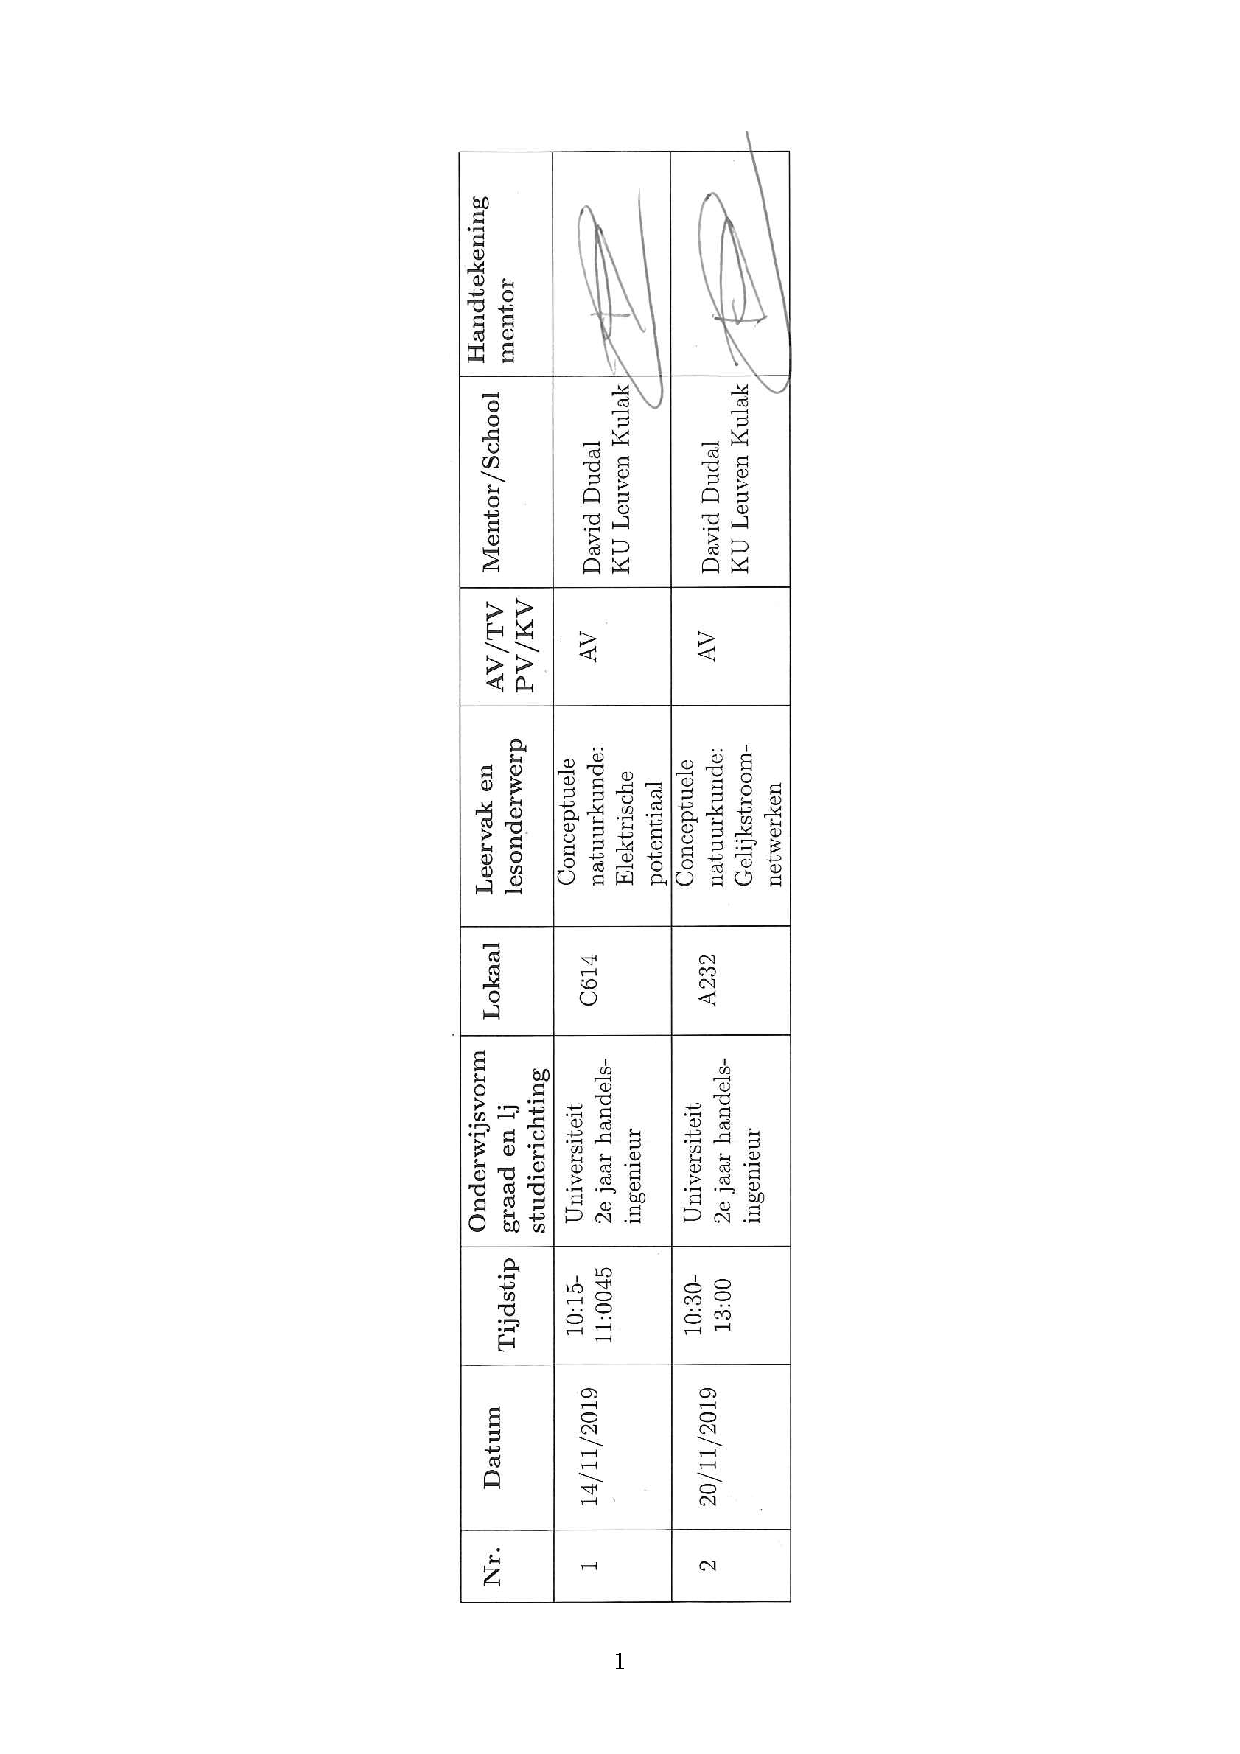
\includegraphics[scale = 0.9,trim={7.8cm 2cm 7.3cm 2cm} ,clip,angle=-90]{OnePageObservatieKulak}
\end{center}
%\end{minipage}

\subsubsection{VISO}%\\
\vspace*{-0.5cm}
\begin{center}
	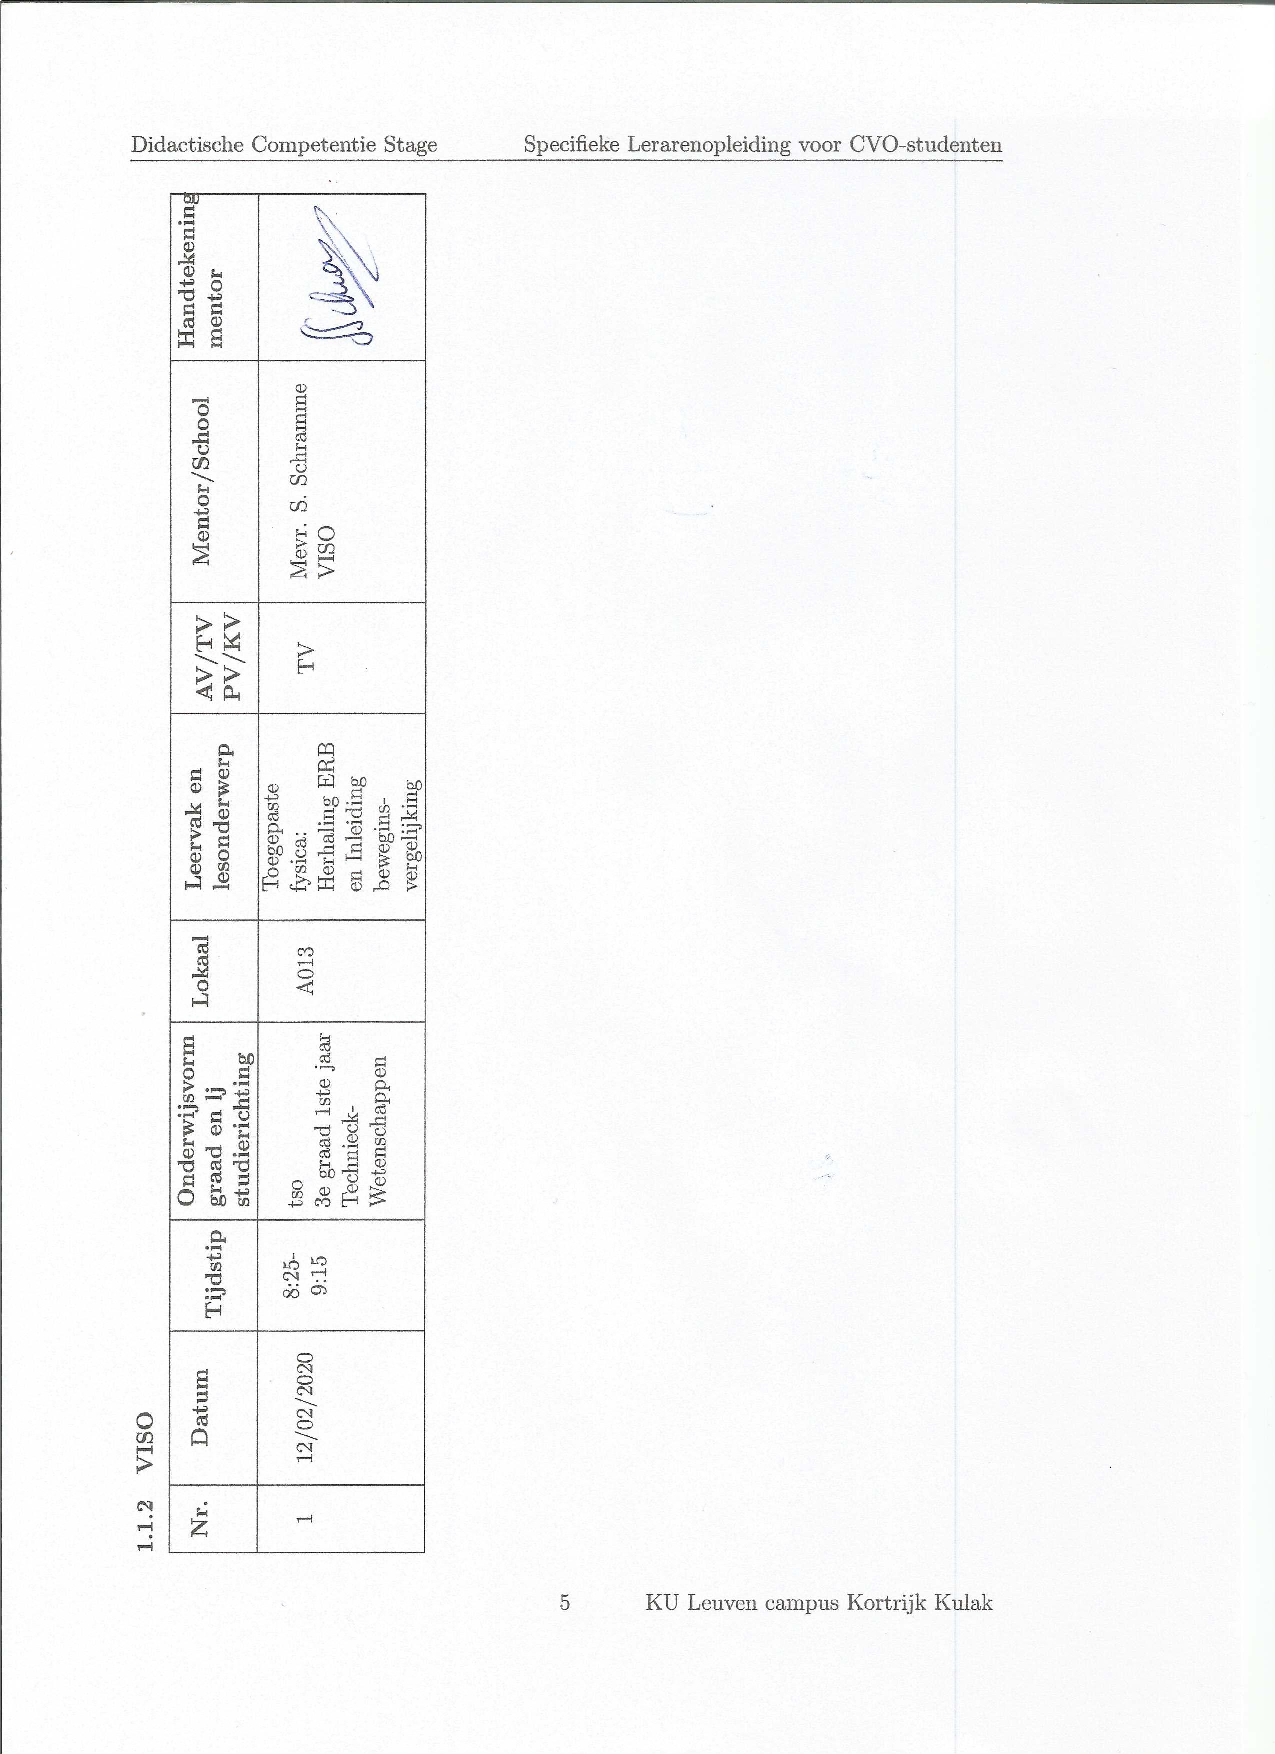
\includegraphics[scale = 0.9,trim={2.8cm 3cm 14.2cm 3cm} ,clip,angle=-90]{ObservatielesVISO}
\end{center}
%\begin{tabularx}{1.56\textwidth}{|C{0.05\textwidth}|C{0.15\textwidth}|C{0.1\textwidth}|C{0.2\textwidth}|C{0.09\textwidth}|C{0.21\textwidth}|C{0.1\textwidth}|C{0.25\textwidth}|X|}
%	\hline
%	\textbf{Nr.} & \textbf{Datum} & \textbf{Tijdstip} & \textbf{\begin{tabular}[C]{@{}l@{}}Onderwijsvorm\\ graad en lj\\ studierichting\end{tabular}} & \textbf{Lokaal} &\textbf{\begin{tabular}[C]{@{}l@{}} Leervak en\\ lesonderwerp \end{tabular}} & \textbf{\begin{tabular}[C]{@{}l@{}}AV/TV\\PV/KV\end{tabular}} & \textbf{Mentor/School} & \textbf{\begin{tabular}[C]{@{}l@{}} Handtekening\\mentor\end{tabular}}\\ \hline
%	1 & 12/02/2020 & 8:25-9:15 &\begin{tabular}[C]{@{}l@{}}tso\\3e graad 1ste jaar\\ Technieck-\\Wetenschappen\\\end{tabular} & A013 & \begin{tabular}[C]{@{}l@{}}Toegepaste\\ fysica:\\ Herhaling ERB\\en Inleiding\\ bewegins-\\vergelijking \end{tabular} & TV & \begin{tabular}[C]{@{}l@{}}Mevr. S. Schramme\\ VISO \end{tabular} & \\ \hline
%\end{tabularx}
	
\newpage
\subsection{Actieve stage}
		\subsubsection{Kulak (LIO)}
	%	
	%	\begin{minipage}[t][10cm][t]{0.5\textwidth}
			\begin{figure*}[h]
				\begin{tikzpicture}
				\node[anchor=south west] 
				at (0,0) %left bottom corner of the page
				{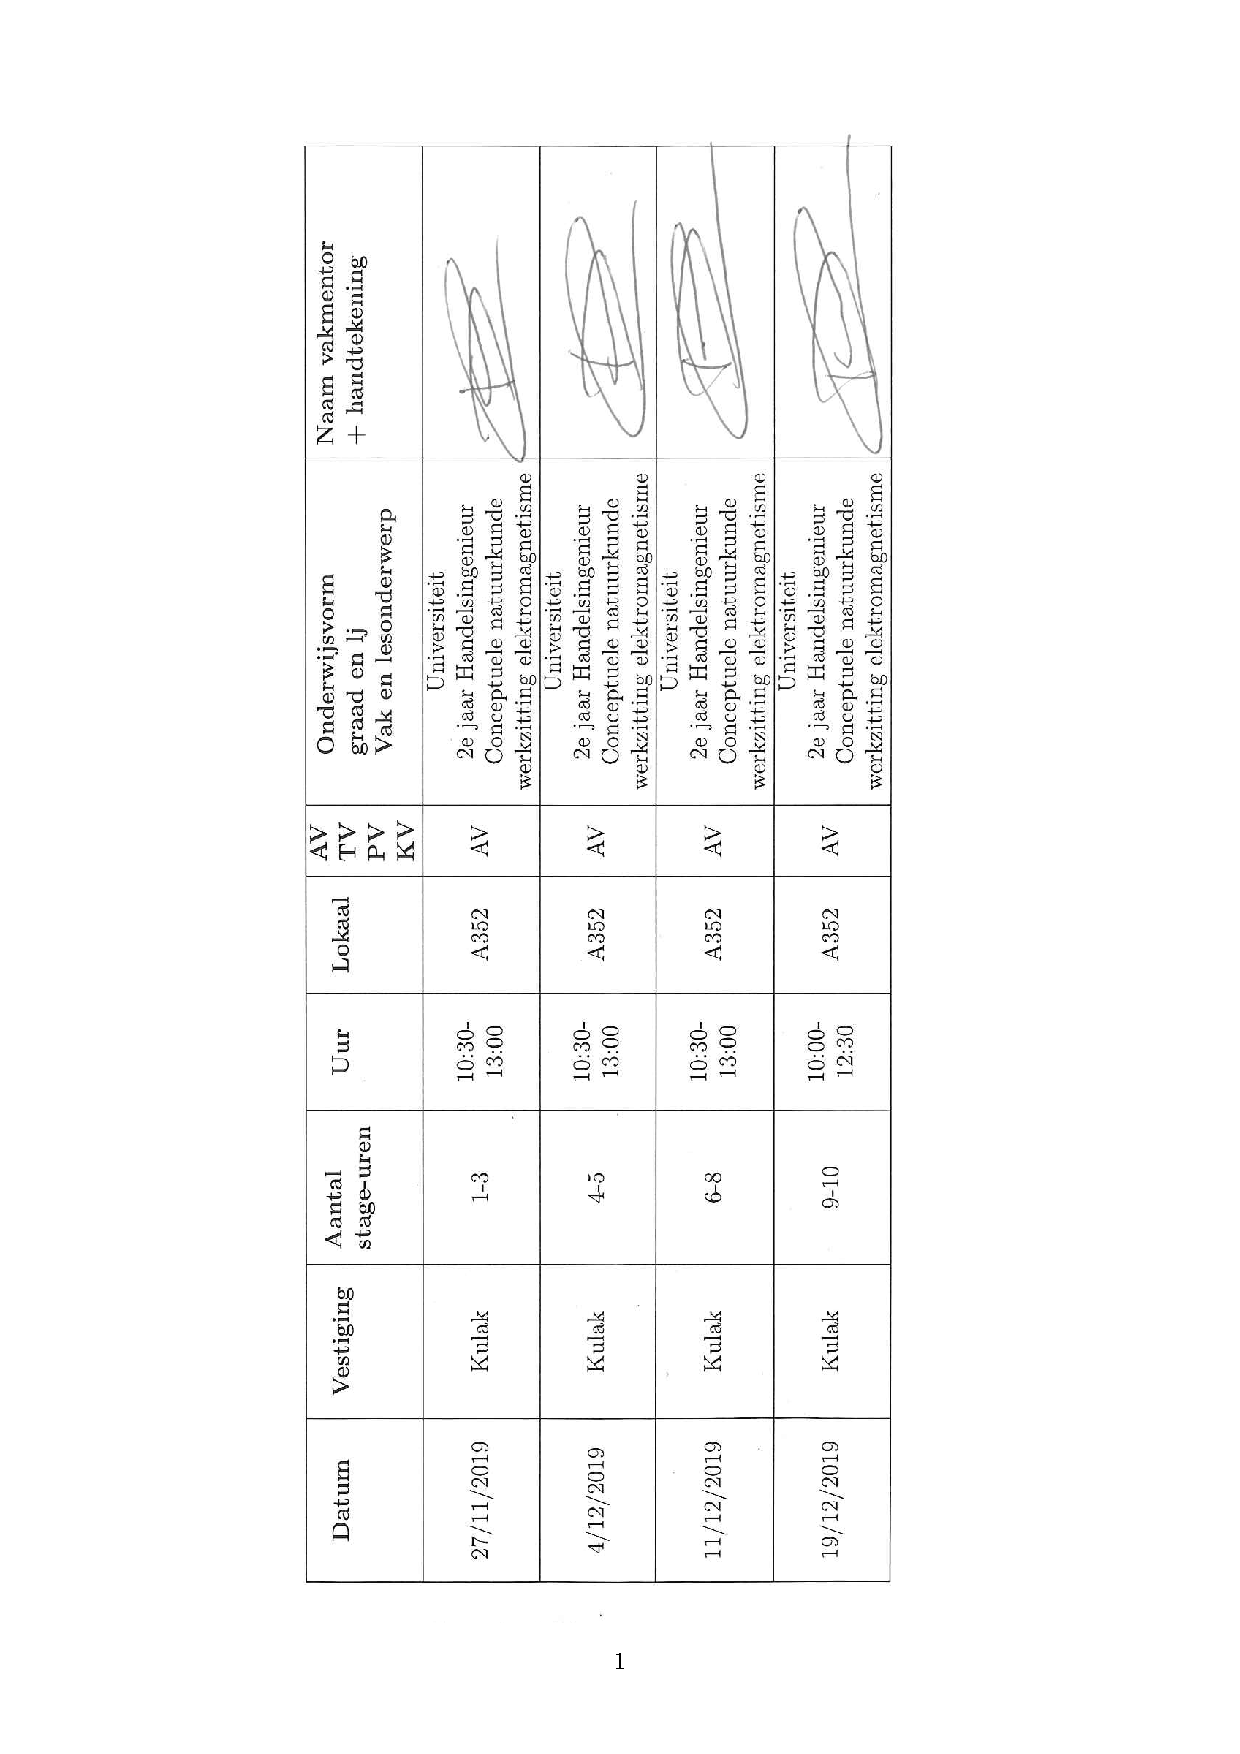
\includegraphics[scale = 0.85,trim={4cm 2cm 6cm 1.8cm} ,clip,angle=-90 ]{OnePageLesgevenKulak}};
				\node[fill=white] at(6.58,4.25){4-6};
				\node[fill=white] at(6.58,2.55){7-9};
				\node[fill=white] at(6.58,0.85){10-12};				
				\end{tikzpicture}
			\end{figure*}
		%\end{minipage}
		\vfill\newpage
%	\begin{tabularx}{1.56\textwidth}{|C{0.15\textwidth}|C{0.14\textwidth}|C{0.14\textwidth}|C{0.1\textwidth}|C{0.1\textwidth}|C{0.05\textwidth}|C{0.35\textwidth}|X|}
%		\hline
%		\textbf{Datum} & \textbf{Vestiging} & \textbf{\begin{tabular}[C]{@{}l@{}}Aantal\\ stage-uren\end{tabular}} & \textbf{\begin{tabular}[C]{@{}l@{}}Uur \end{tabular}}    & \textbf{Lokaal}& \textbf{\begin{tabular}[C]{@{}l@{}}AV\\TV\\PV\\KV\end{tabular}}& \textbf{\begin{tabular}[C]{@{}l@{}}Onderwijsvorm\\ graad en lj\\ Vak en lesonderwerp\end{tabular}}  &  \textbf{\begin{tabular}[C]{@{}l@{}}Naam vakmentor\\ + handtekening\end{tabular} } \\ \hline
%		27/11/2019 & Kulak & 1-3 & 10:30-13:00 & A352 & AV & Universiteit\newline 2e jaar Handelsingenieur\newline Conceptuele natuurkunde\newline werkzitting elektromagnetisme & \\ 
%\hline
%		4/12/2019 & Kulak & 4-5 & 10:30-13:00 & A352 & AV & Universiteit\newline 2e jaar Handelsingenieur\newline Conceptuele natuurkunde\newline werkzitting elektromagnetisme & \\ \hline
%		11/12/2019 & Kulak & 6-8 & 10:30-13:00 & A352 & AV & Universiteit\newline 2e jaar Handelsingenieur\newline Conceptuele natuurkunde\newline werkzitting elektromagnetisme & \\ \hline
%		19/12/2019 & Kulak & 9-10 & 10:00-12:30 & A352 & AV & Universiteit\newline 2e jaar Handelsingenieur\newline Conceptuele natuurkunde\newline werkzitting elektromagnetisme & \\ \hline
%	%	 &  &  &  &  &  &  & \\ \hline
%	\end{tabularx}
%	
\subsubsection{VISO Roeselare}

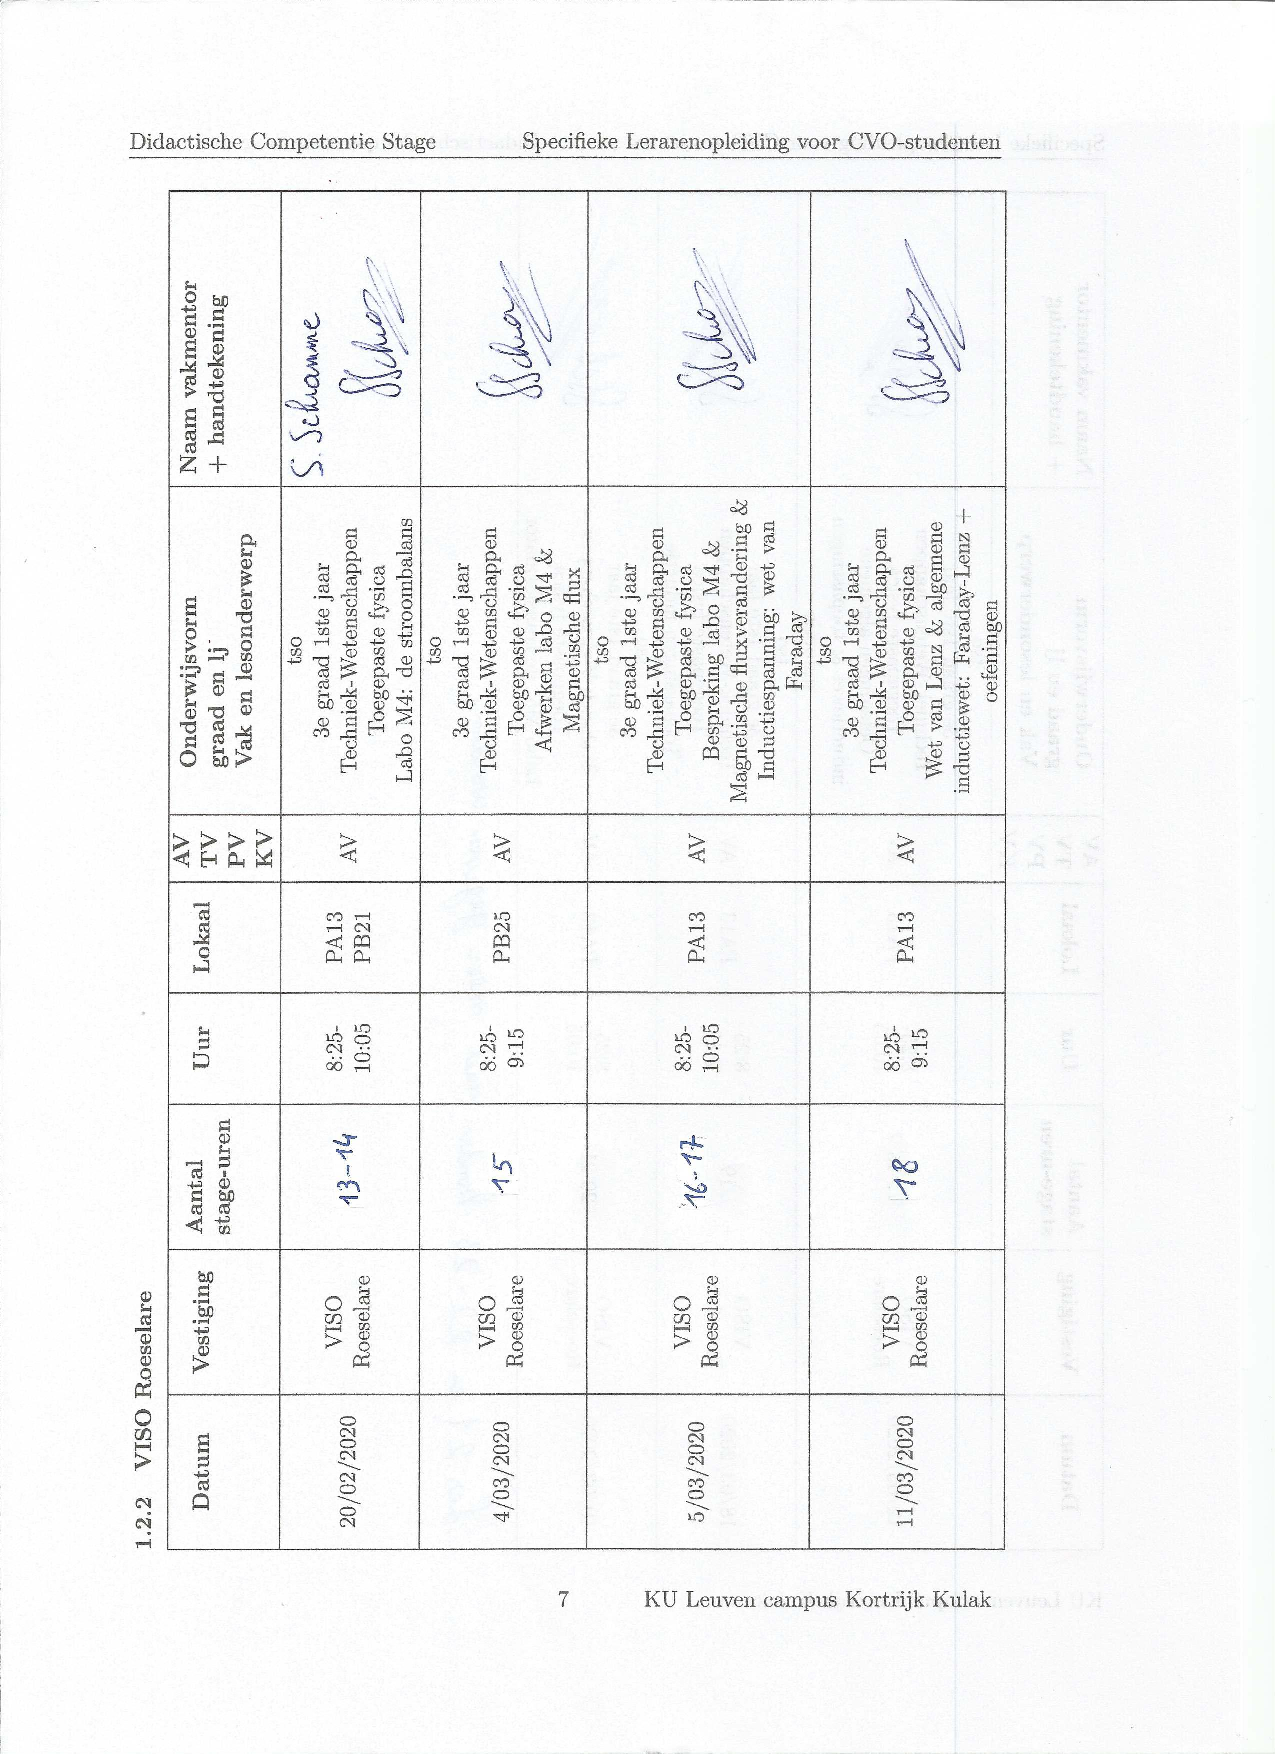
\includegraphics[scale = 0.95,trim={2.7cm 3cm 4cm 3cm} ,clip,angle=-90 ]{P1PlanningVISO}\newpage
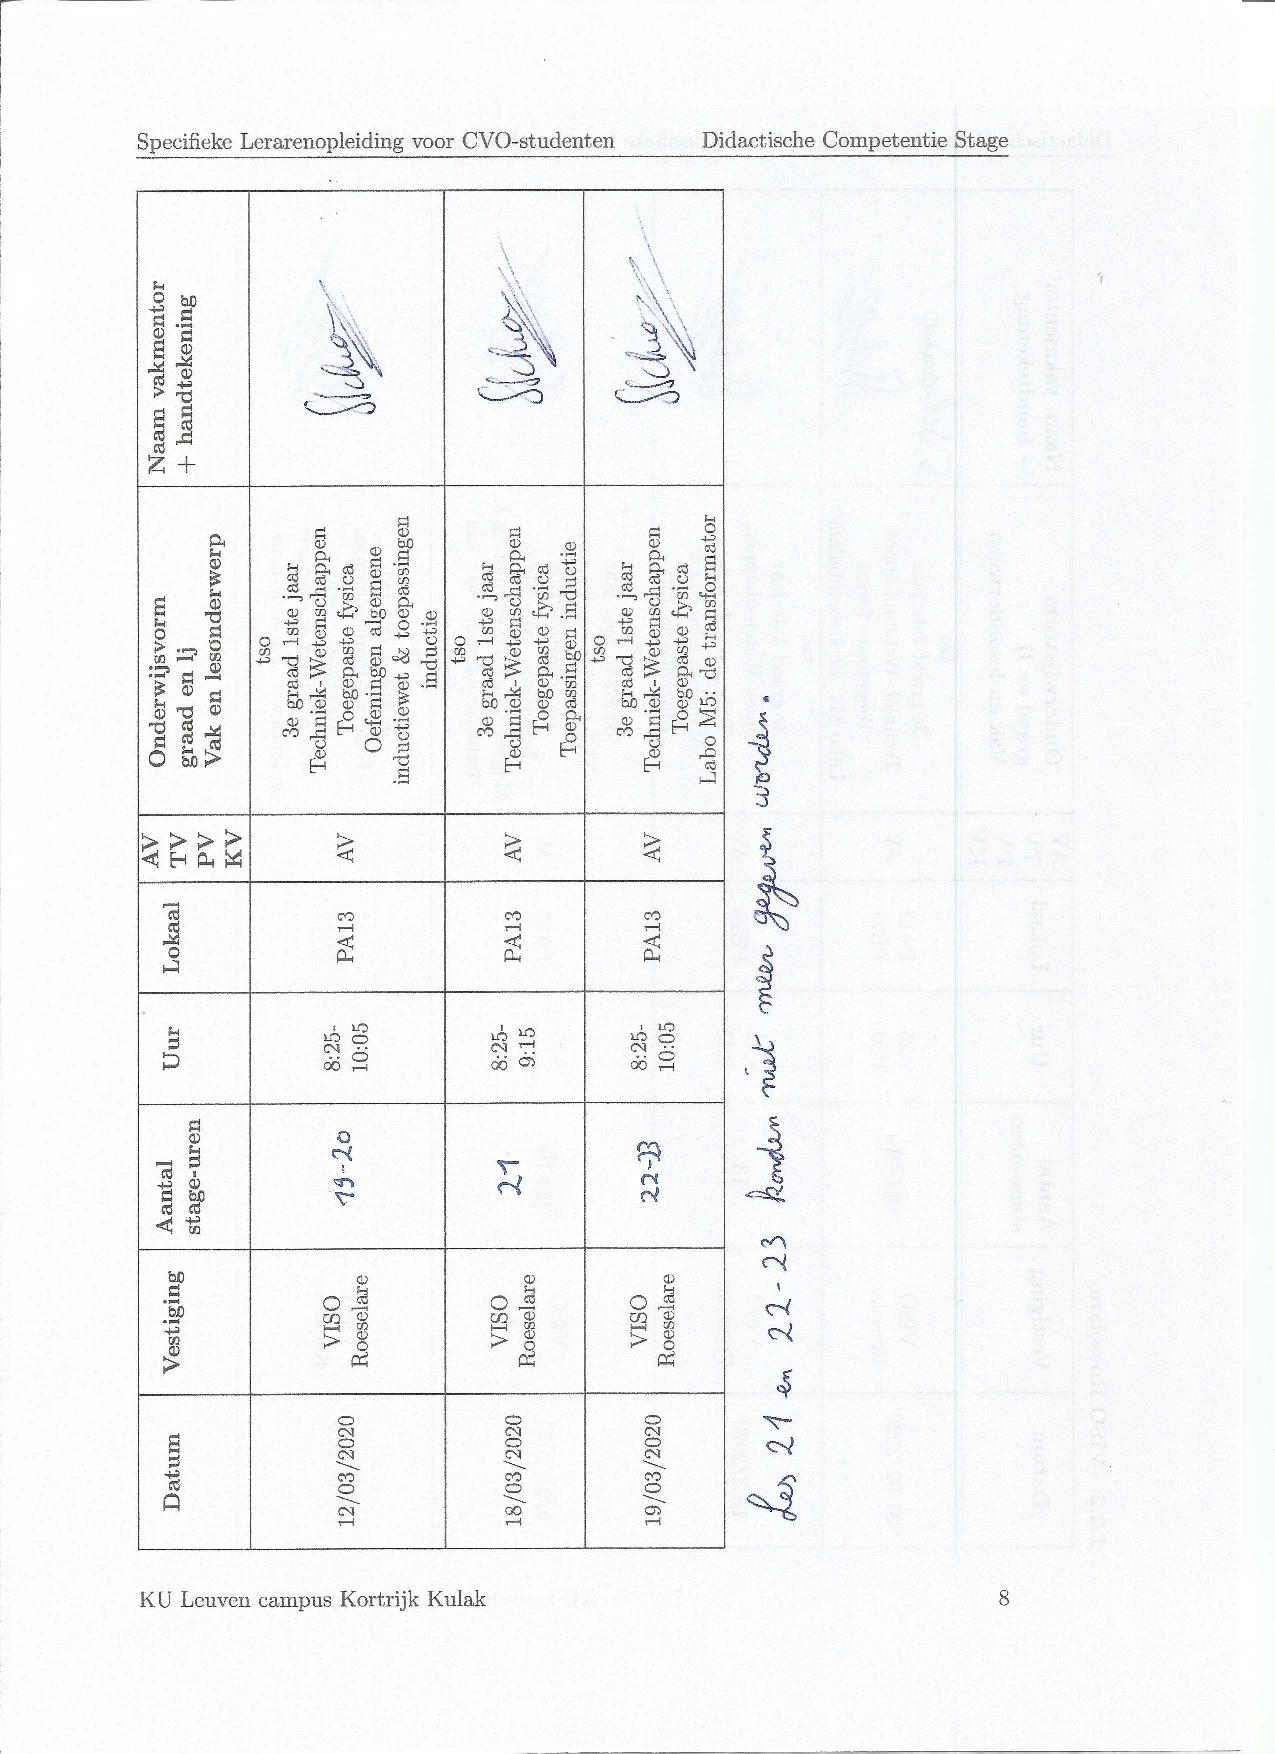
\includegraphics[scale = 0.95,trim={2cm 3cm 8cm 3cm} ,clip,angle=-90 ]{P2PlanningVISO}
%\begin{tabularx}{1.56\textwidth}{|C{0.15\textwidth}|C{0.14\textwidth}|C{0.14\textwidth}|C{0.1\textwidth}|C{0.1\textwidth}|C{0.05\textwidth}|C{0.35\textwidth}|X|}
%	\hline
%	\textbf{Datum} & \textbf{Vestiging} & \textbf{\begin{tabular}[C]{@{}l@{}}Aantal\\ stage-uren\end{tabular}} & \textbf{\begin{tabular}[C]{@{}l@{}}Uur \end{tabular}}    & \textbf{Lokaal}& \textbf{\begin{tabular}[C]{@{}l@{}}AV\\TV\\PV\\KV\end{tabular}}& \textbf{\begin{tabular}[C]{@{}l@{}}Onderwijsvorm\\ graad en lj\\ Vak en lesonderwerp\end{tabular}}  &  \textbf{\begin{tabular}[C]{@{}l@{}}Naam vakmentor\\ + handtekening\end{tabular} } \\ \hline
%	20/02/2020 & VISO Roeselare & 11-12 & 8:25-10:05 & PA13\newline PB21 & AV & tso\newline 3e graad 1ste jaar Techniek-Wetenschappen\newline Toegepaste fysica\newline Labo M4: de stroombalans & \\ \hline
%	4/03/2020 & VISO Roeselare & 13 & 8:25-9:15 & PB25 & AV & tso\newline 3e graad 1ste jaar Techniek-Wetenschappen\newline Toegepaste fysica\newline Afwerken labo M4  \&\newline Magnetische flux& \\ \hline
%	5/03/2020 & VISO Roeselare & 14-15 & 8:25-10:05 & PA13 & AV & tso\newline 3e graad 1ste jaar Techniek-Wetenschappen\newline Toegepaste fysica\newline Bespreking labo M4 \& Magnetische fluxverandering \& Inductiespanning: wet van Faraday  & \\ \hline
%	11/03/2020 & VISO Roeselare & 16 & 8:25-9:15 & PA13 & AV & tso\newline 3e graad 1ste jaar Techniek-Wetenschappen\newline Toegepaste fysica\newline  Wet van Lenz \& algemene inductiewet: Faraday-Lenz + oefeningen  & \\ \hline
%\end{tabularx}\newpage
%\begin{tabularx}{1.56\textwidth}{|C{0.15\textwidth}|C{0.14\textwidth}|C{0.14\textwidth}|C{0.1\textwidth}|C{0.1\textwidth}|C{0.05\textwidth}|C{0.35\textwidth}|X|}
%	\hline
%	\textbf{Datum} & \textbf{Vestiging} & \textbf{\begin{tabular}[C]{@{}l@{}}Aantal\\ stage-uren\end{tabular}} & \textbf{\begin{tabular}[C]{@{}l@{}}Uur \end{tabular}}    & \textbf{Lokaal}& \textbf{\begin{tabular}[C]{@{}l@{}}AV\\TV\\PV\\KV\end{tabular}}& \textbf{\begin{tabular}[C]{@{}l@{}}Onderwijsvorm\\ graad en lj\\ Vak en lesonderwerp\end{tabular}}  &  \textbf{\begin{tabular}[C]{@{}l@{}}Naam vakmentor\\ + handtekening\end{tabular} } \\ \hline
%	12/03/2020 & VISO Roeselare & 17-18 & 8:25-10:05 & PA13 & AV & tso\newline 3e graad 1ste jaar Techniek-Wetenschappen\newline Toegepaste fysica\newline Oefeningen algemene inductiewet \& toepassingen inductie & \\ \hline
%	18/03/2020 & VISO Roeselare & 19 & 8:25-9:15 & PA13 & AV & tso\newline 3e graad 1ste jaar Techniek-Wetenschappen\newline Toegepaste fysica\newline Toepassingen inductie & \\ \hline
%	19/03/2020 & VISO Roeselare & 20-21 & 8:25-10:05 & PA13 & AV & tso\newline 3e graad 1ste jaar Techniek-Wetenschappen\newline Toegepaste fysica\newline Labo M5: de transformator  & \\ 
%\hline	
%%	 &  &  &  &  &  &  & \\ \hline
%\end{tabularx}
	


		
\end{landscape}		
		
